\section{Phương pháp nghiên cứu} % section 3

\subsection{Thiết kế nghiên cứu} % section 3.1
Nghiên cứu được thiết kế theo phương pháp định lượng, tập trung vào việc xây dựng và đánh giá hiệu suất của các mô hình học sâu trong bài toán nhận diện biểu cảm khuôn mặt (Facial Expression Recognition - FER) trong điều kiện ánh sáng yếu. Phương pháp định lượng được chọn vì mục tiêu nghiên cứu là đo lường các chỉ số hiệu suất cụ thể (Accuracy, Precision, Recall, F1-score và thời gian suy luận) của hai mô hình CNN: MobileNetV3 (mô hình nhẹ) và ResNet18 (mô hình sâu hơn), khi áp dụng kỹ thuật tăng cường dữ liệu thích ứng.

Quá trình nghiên cứu bao gồm ba giai đoạn chính:
\begin{itemize}
    \item \textbf{Tiền xử lý dữ liệu:} Sử dụng tập dữ liệu FER-2013, áp dụng các kỹ thuật tăng cường dữ liệu thích ứng để mô phỏng điều kiện ánh sáng yếu.
    \item \textbf{Huấn luyện và tối ưu mô hình:} Triển khai MobileNetV3 và ResNet18, tinh chỉnh các tham số để phù hợp với bài toán FER.
    \item \textbf{Đánh giá và so sánh:} So sánh hiệu suất và thời gian suy luận của các mô hình khi có và không áp dụng kỹ thuật tăng cường dữ liệu thích ứng.
\end{itemize}

\subsection{Đối tượng và mẫu nghiên cứu} % section 3.2
\subsubsection{Đối tượng nghiên cứu} % section 3.2.1
Đối tượng nghiên cứu là các kỹ thuật nhận diện biểu cảm khuôn mặt trong điều kiện ánh sáng yếu, với trọng tâm vào:
\begin{itemize}
    \item \textbf{Mô hình học sâu:} MobileNetV3 và ResNet18 dùng để phân loại 7 biểu cảm khuôn mặt (vui, buồn, tức giận, sợ hãi, ngạc nhiên, ghê tởm, trung lập).
    \item \textbf{Kỹ thuật tăng cường dữ liệu thích ứng:} Các phương pháp như gamma correction, contrast stretching và histogram equalization, được điều chỉnh dựa trên đặc trưng ánh sáng của hình ảnh.
\end{itemize}

\subsubsection{Mẫu nghiên cứu} % section 3.2.2
Mẫu nghiên cứu là tập dữ liệu FER-2013, chứa 35.887 hình ảnh khuôn mặt (48x48 pixel, ảnh xám) được phân loại thành 7 biểu cảm. Tập dữ liệu được chia như sau:
\begin{itemize}
    \item Tập huấn luyện: 28.709 hình ảnh (~80\%).
    \item Tập xác thực (validation): 3.589 hình ảnh (~10.00\%).
    \item Tập kiểm tra: 3.589 hình ảnh (~10.00\%).
\end{itemize}

Nhằm mô phỏng điều kiện ánh sáng yếu, một tập dữ liệu phụ được tạo ra bằng cách giảm độ sáng của ảnh gốc. Quá trình này thực hiện bằng cách chuyển ảnh sang không gian màu HSV, giảm kênh độ sáng (V) theo một hệ số cố định, sau đó chuyển lại về không gian RGB. Cụ thể, độ sáng được giảm xuống 10\% so với ảnh ban đầu.





\subsection{Cách thu thập dữ liệu} % section 3.3
Dữ liệu được thu thập từ tập dữ liệu FER-2013 công khai trên nền tảng Kaggle. Các bước gồm:

\subsubsection*{Thu thập dữ liệu}
\begin{itemize}
    \item Tải tập dữ liệu FER-2013 từ Kaggle.
    \item Kiểm tra tính toàn vẹn (số lượng ảnh, định dạng, chất lượng).
\end{itemize}

\subsubsection{EDA dữ liệu} % section 3.2.3
Phân tích dữ liệu khám phá (EDA) được thực hiện trên tập dữ liệu FER-2013 nhằm hiểu rõ cấu trúc, phân phối và đặc trưng của dữ liệu trước khi áp dụng các mô hình học sâu. Dữ liệu được lưu trữ dưới dạng tệp CSV với ba cột chính: cột \texttt{emotion} (nhãn cảm xúc, giá trị từ 0 đến 6), cột \texttt{pixels} (tập hợp các giá trị pixel của ảnh dưới dạng chuỗi số), và cột \texttt{Usage} (chỉ định tập huấn luyện, xác thực hoặc kiểm tra). Kích thước tổng cộng của tập dữ liệu là 35.887 mẫu, trong đó mỗi hình ảnh có độ phân giải 48x48 pixel.


\begin{figure}[H]
    \centering
    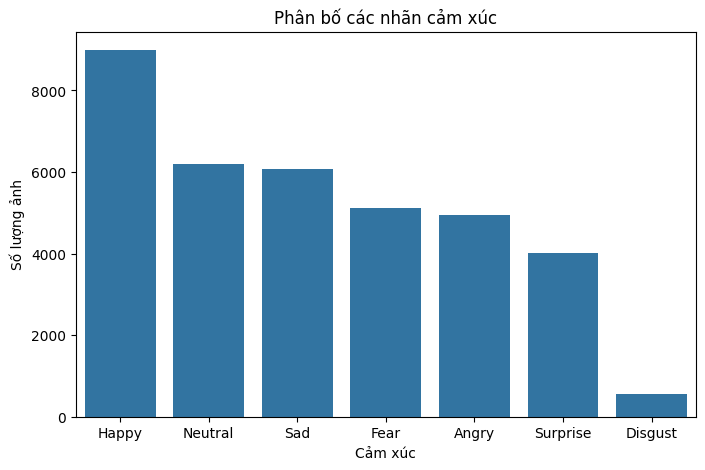
\includegraphics[width=0.7\textwidth]{img/phan_bo_nhan_cam_xuc.png} % Đường dẫn tương đối
    \caption{Phân bố nhãn cảm xúc trong tập dữ liệu FER-2013.}
    \label{fig:emotion_distribution}
    \par\vspace{0.5cm} % Khoảng cách giữa hình và ý nghĩa
    \textit{Ý nghĩa:} 
\end{figure}

\begin{figure}[H]
    \centering
    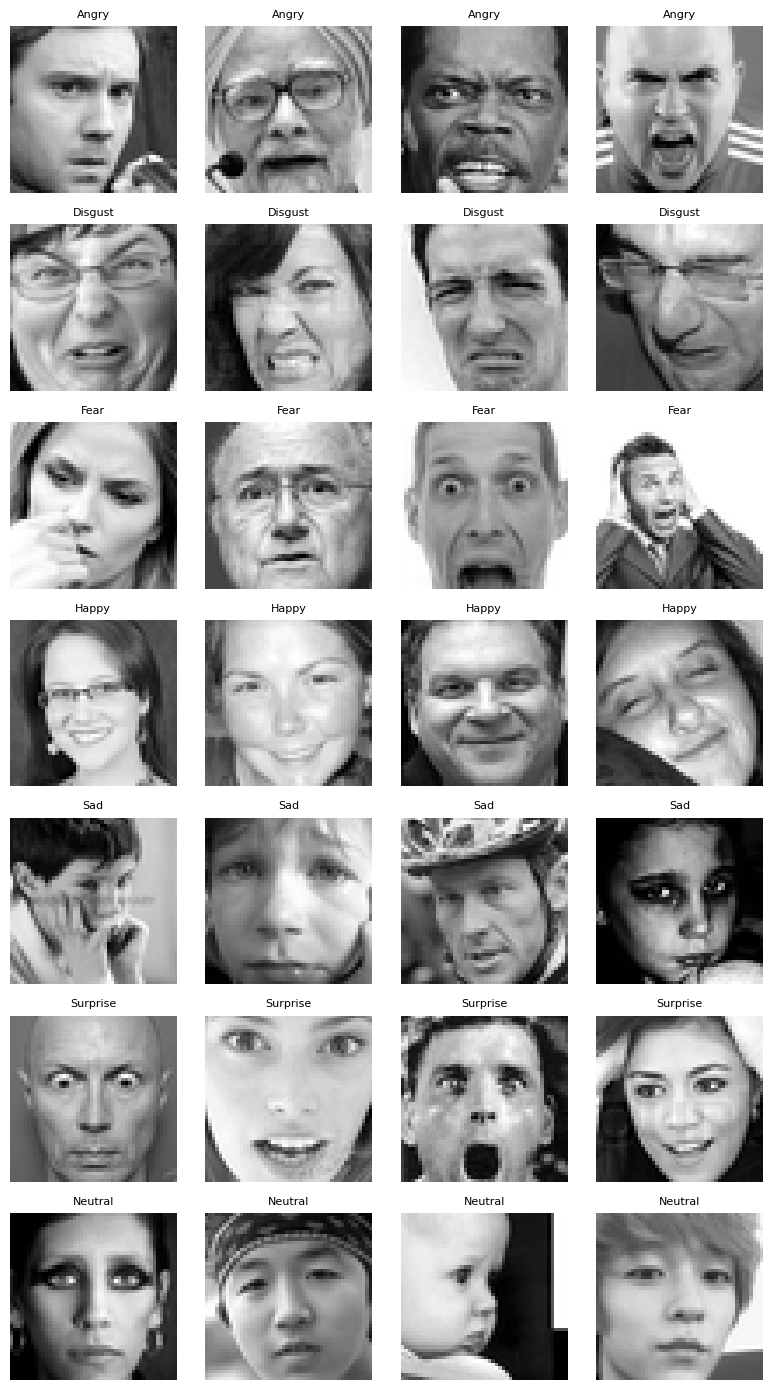
\includegraphics[width=0.7\textwidth]{img/truc_quan_anh_mau.png} % Đường dẫn tương đối
    \caption{Một số hình ảnh mẫu từ tập dữ liệu FER-2013.}
    \label{fig:sample_images}
    \par\vspace{0.5cm} % Khoảng cách giữa hình và ý nghĩa
    \textit{Ý nghĩa:} 
\end{figure}

\begin{figure}[H]
    \centering
    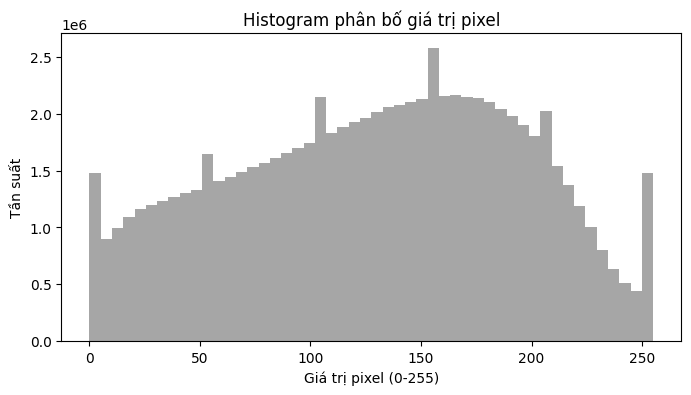
\includegraphics[width=0.7\textwidth]{img/phan_bo_pixel.png} % Đường dẫn tương đối
    \caption{Phân bố pixel trong tập dữ liệu FER-2013.}
    \label{fig:pixel_distribution}
    \par\vspace{0.5cm} % Khoảng cách giữa hình và ý nghĩa
    \textit{Ý nghĩa:} 
\end{figure}

\begin{figure}[H]
    \centering
    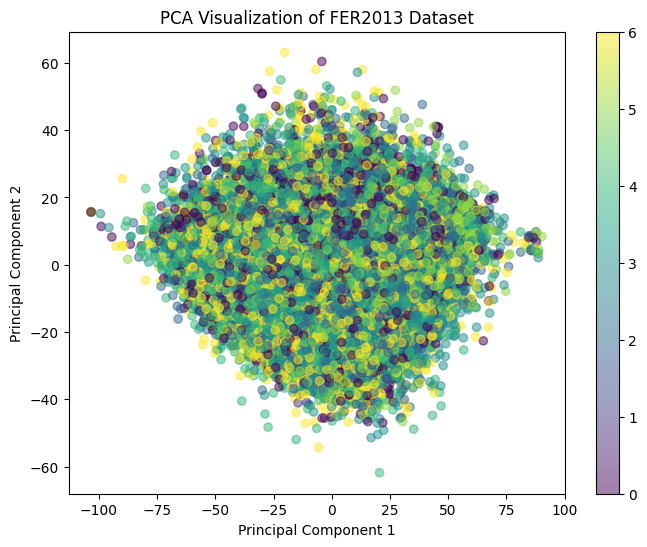
\includegraphics[width=0.7\textwidth]{img/PCA.png} % Đường dẫn tương đối
    \caption{Trực quan hóa dữ liệu FER-2013 bằng PCA.}
    \label{fig:pca_visualization}
    \par\vspace{0.5cm} % Khoảng cách giữa hình và ý nghĩa
    \textit{Ý nghĩa:} 
\end{figure}


\subsubsection{Tiền xử lý dữ liệu}

Các bước tiền xử lý được thực hiện nhằm cải thiện chất lượng ảnh đầu vào và mô phỏng các điều kiện môi trường khác nhau, cụ thể như sau:

\begin{itemize}
    \item \textbf{Chuẩn hóa hình ảnh}: Loại bỏ nhiễu và đảm bảo định dạng đồng nhất (kích thước ảnh, không gian màu), giúp mô hình huấn luyện ổn định hơn.
    
    \item \textbf{Mô phỏng điều kiện ánh sáng yếu}: Để mô phỏng môi trường có ánh sáng yếu, hình ảnh được chuyển sang không gian màu HSV và kênh độ sáng (V) được giảm xuống còn 10\% so với ảnh gốc. Sau đó, ảnh được chuyển lại về không gian RGB để sử dụng trong huấn luyện.
\end{itemize}

\subsubsection{Tăng cường dữ liệu thích ứng}
Áp dụng các phép biến đổi linh hoạt dựa trên đặc trưng ánh sáng của từng ảnh. Việc tăng cường được thực hiện bằng Python với OpenCV và NumPy.

\subsection{Phân tích dữ liệu}
\subsubsection{Công cụ và phần mềm}
\begin{itemize}
    \item Python: xử lý dữ liệu và huấn luyện mô hình.
    \item PyTorch : xử lý dữ liệu và huấn luyện mô hình.
    \item TensorFlow/Keras: xây dựng và đánh giá mô hình.
    \item OpenCV: tiền xử lý ảnh.
    \item NumPy, Pandas: quản lý dữ liệu.
    \item Matplotlib, Seaborn: trực quan hóa kết quả.
\end{itemize}

\subsubsection{Quy trình phân tích}
\begin{itemize}
    \item \textbf{Huấn luyện mô hình MobileNetV3Small:}
    \begin{itemize}
        \item Sử dụng mô hình MobileNetV3Small với trọng số ImageNet, loại bỏ phần fully-connected gốc (include\_top=False).
        \item Chỉ tinh chỉnh 30 lớp cuối cùng trong mạng, các lớp còn lại được đóng băng để giữ lại đặc trưng đã học.
        \item Kiến trúc phần đầu ra gồm: Global Average Pooling, hai lớp Dense (128 và 64 nodes, activation ReLU), kèm Dropout 0.3, kết thúc bằng lớp Softmax với 7 nhãn đầu ra.
        \item Hàm mất mát: Categorical Crossentropy.
        \item Tối ưu hóa bằng Adam (learning rate mặc định).
        \item Số epoch: 10, sử dụng Early Stopping với patience = 3 để tránh overfitting.
    \end{itemize}

    \item \textbf{Huấn luyện mô hình với ResNet18:}
    \begin{itemize}
        \item Sử dụng mô hình \textbf{ResNet18} với trọng số đã được huấn luyện sẵn trên tập ImageNet (\texttt{ResNet18\_Weights.IMAGENET1K\_V1}).
        \item Điều chỉnh lại lớp Fully Connected cuối cùng thành \texttt{nn.Linear(..., 7)} để phù hợp với bài toán phân loại 7 cảm xúc trên tập dữ liệu FER2013.
        \item Hàm mất mát sử dụng là \textbf{CrossEntropyLoss}, phù hợp với phân loại đa lớp.
        \item Trình tối ưu hóa: \textbf{Adam} với learning rate 0.001.
        \item Mô hình được huấn luyện trong \textbf{20 epoch}.
        \item Trong quá trình huấn luyện, độ chính xác và mất mát (loss) trên tập huấn luyện và tập xác thực được theo dõi để đánh giá hiệu quả mô hình. Mô hình tốt nhất được lưu lại sau mỗi epoch nếu có cải thiện.
    \end{itemize}

    \item \textbf{Đánh giá mô hình:}
    \begin{itemize}
        \item Các chỉ số đánh giá: Accuracy, Precision, Recall, F1-score.
        \item Đo thời gian suy luận trung bình trên CPU (per image).
        \item Kích cỡ mô hình sau huấn luyện.
    \end{itemize}

    \item \textbf{So sánh mô hình:}
    \begin{itemize}
        \item MobileNetV3 (cơ bản vs. tăng cường).
        \item ResNet18 (cơ bản vs. tăng cường).
        \item So sánh giữa MobileNetV3 và ResNet18.
    \end{itemize}
    
    \item \textbf{Phân tích kết quả:}
    \begin{itemize}
        \item Ma trận nhầm lẫn, biểu đồ Accuracy theo epoch.
        \item Quan sát các trường hợp dự đoán sai.
    \end{itemize}
\end{itemize}

\subsubsection{Thiết bị triển khai}
Thực nghiệm được thực hiện trên máy MacBook Air M1, được trang bị chip Apple M1 và RAM 8GB. Ngoài ra, Google Colab cũng được sử dụng để mô phỏng điều kiện tài nguyên thấp, với việc chỉ sử dụng CPU thay vì GPU nhằm đánh giá thời gian suy luận, phù hợp với môi trường nhúng.

\subsection{Phương pháp so sánh}
Nghiên cứu tiến hành so sánh định lượng qua các chỉ số hiệu suất (Accuracy, Precision, Recall, F1-score) và thời gian suy luận giữa:
\begin{itemize}
    \item MobileNetV3 cơ bản vs. tăng cường.
    \item ResNet18 cơ bản vs. tăng cường.
    \item So sánh giữa MobileNetV3 và ResNet18.
\end{itemize}

Kết quả được trình bày dưới dạng bảng và biểu đồ để làm rõ hiệu quả của các kỹ thuật và sự phù hợp của mô hình trong ứng dụng thực tế.